\chapter{Control Architecture}
\section{Control Objectives}
The objective of the control strategy is to regulate the motion of the hand exoskeleton in a compliant and stable manner during interaction with the user. In rehabilitation scenarios, the device must not impose a predefined motion trajectory rigidly, but instead adapt its behavior in response to externally applied forces. This requirement motivates the adoption of an admittance control framework, in which the motion of the system is determined by the interaction forces rather than being directly prescribed.
From a control perspective, the Digital Twin developed in this work provides a reduced-order dynamic model of the form:

\begin{equation}
    I_{eff}(\theta)\ddot{\theta} = \tau_m + \tau_{pass,\theta} + \tau_{ext,\theta} - p(\theta, \dot{\theta}) - \tau_{fric} - \tau_{damp}
\end{equation}

where $I_{eff}(\theta) = B^T M(q)\,B + J_m$ is the effective inertia augmented by the motor rotor inertia $J_m$, $p = B^T\!\bigl(M\,\dot B\,\dot\theta + h\bigr)$ collects the projected Coriolis, centrifugal, gravitational and geometric-acceleration contributions, $\tau_{\mathrm{fric}}$ accounts for viscous and Coulomb friction, $\tau_{\mathrm{damp}}$ represents an additional viscous damping term on the reduced coordinate, $\tau_{\mathrm{pass},\theta}$ is the projected passive biomechanical torque, and $\tau_{\mathrm{ext},\theta}$ is the projected external interaction torque.

The control objective is therefore to compute the motor torque $\tau_m$ such that the system exhibits a desired compliant behavior with respect to external interaction forces.

The control architecture adopted in this work follows a hierarchical structure composed of two nested control loops. The outer loop regulates the interaction behavior between the user and the exoskeleton by generating a desired motion trajectory based on the measured interaction forces. The inner loop ensures accurate tracking of this desired motion by compensating for the nonlinear dynamics of the system. This separation enables the system to achieve compliant interaction at the high level while maintaining precise and stable motion control at the low level.

\begin{figure}[ht]
    \centering
    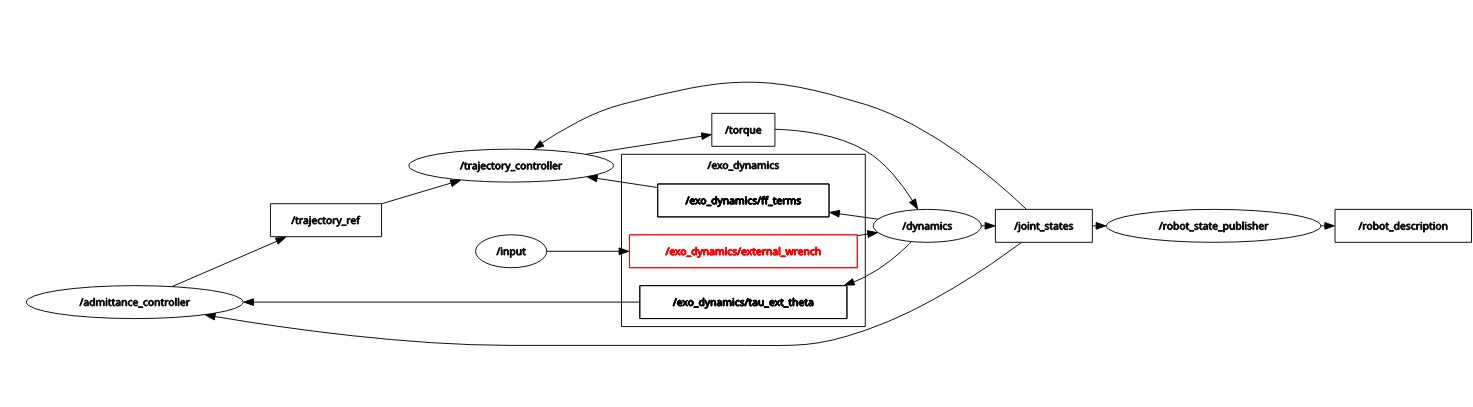
\includegraphics[scale=0.35]{images/chapter4/control_loop_rqt_graph.png}
    \caption{Control Loop rqt\_graph}
    \label{fig:control_loop_rqt_graph}
\end{figure}
\FloatBarrier

\section{Outer Loop: Admittance Control}
In physical human–robot interaction, two dual approaches exist for regulating the contact behavior: impedance control, in which the robot modulates force in response to a prescribed motion deviation, and admittance control, in which the robot modulates motion in response to a measured force. In the admittance paradigm, the desired interaction behaviour is encoded in a virtual mechanical model of the form:

\begin{equation}
M_v\,\ddot\theta_v + D_v\,\dot\theta_v + K_v\,(\theta_v - \theta_{\mathrm{eq}})
  = \tau_{\mathrm{in}}
\end{equation}

where $\theta_v$ is the virtual coordinate whose evolution constitutes the position reference for the inner control loop, $\tau_{\mathrm{in}}$ is the filtered generalized force applied by the user (defined below), and $M_v$, $D_v$ and $K_v$ are the virtual inertia, damping, and stiffness respectively. The equilibrium position $\theta_{\mathrm{eq}}$ defines the resting configuration toward which the spring term drives the system in the absence of user input. This formulation is deliberately independent of the physical inertia and stiffness of the mechanism: the virtual parameters $(M_v, D_v, K_v)$ are design choices that shape the perceived compliance of the device as experienced by the user, and can be tuned freely without altering the underlying plant model.

The rationale for placing this model as an outer loop is rooted in the cascade control philosophy. The admittance controller does not compute a torque command directly; instead, it integrates the virtual dynamics to produce the trajectory $(\theta_v, \dot\theta_v, \ddot\theta_v)$ that represents the desired kinematic response of the mechanism to the user's force. This trajectory is then passed to the inner-loop trajectory controller, which is responsible for commanding the actuator torque required to track it. The separation is beneficial for two reasons: it decouples the interaction design — expressed entirely in the virtual domain through $(M_v, D_v, K_v)$ — from the low-level actuator regulation problem; and it allows each loop to be designed and tuned independently, provided that the inner loop is sufficiently faster than the outer one to be considered transparent from the admittance perspective.

\subsection{Virtual Dynamics and Their Mechanical Interpretation}
The virtual model governing the outer loop is a second-order linear ODE. Rewriting it in standard form:

\begin{equation}
    \ddot\theta_v
  = \frac{\tau_{\mathrm{in}} - D_v\,\dot\theta_v - K_v\,(\theta_v - \theta_{\mathrm{eq}})}{M_v}
\end{equation}

the solution $\theta_v(t)$ describes how a fictitious mechanical system with inertia $M_v$, damping $D_v$, and stiffness $K_v$ would move in response to the external force $\tau_{\mathrm{in}}$.
 
The three virtual parameters shape the interaction behaviour in physically interpretable ways.
 
The virtual inertia $M_v$ determines the sluggishness of the response: a large $M_v$ makes the reference evolve slowly even under large forces, yielding a heavy, inert feel; a small $M_v$ makes the reference react promptly to even small perturbations, yielding a light, responsive behaviour. Crucially, $M_v$ is entirely decoupled from the actual mechanical inertia of the exoskeleton $I_{\mathrm{eff}}(\theta)$, which is in general configuration-dependent and not directly perceptible by the user once the inner loop closes around it.
 
The virtual damping $D_v$ dissipates energy from the virtual system, preventing oscillatory responses and ensuring that the reference trajectory settles smoothly after a force perturbation is removed. From the user's perspective, a large $D_v$ makes the device feel viscous and resistive to fast motions, while a small $D_v$ makes it feel more frictionless. In the rehabilitation context, an appropriately tuned damping term also serves as a safety mechanism: by limiting the rate at which the reference position can change, it bounds the velocity commands issued to the inner loop regardless of the magnitude of the applied force.
 
The virtual stiffness $K_v$ introduces a restoring torque proportional to the displacement of $\theta_v$ from the equilibrium position $\theta_{\mathrm{eq}}$. In the absence of user interaction ($\tau_{\mathrm{in}} = 0$), the virtual system converges exponentially back to $\theta_{\mathrm{eq}}$, with a time constant determined by the ratio $M_v/K_v$ and the natural frequency $\omega_n = \sqrt{K_v/M_v}$. This term is particularly relevant in the context of assisted rehabilitation: by positioning $\theta_{\mathrm{eq}}$ at a target joint angle and selecting an appropriate stiffness $K_v$, the device can provide a gentle assistive torque that encourages the user to move toward the desired configuration, while still allowing them to deviate from it if they are able to do so. Setting $K_v = 0$ yields a purely inertia–damper behaviour, in which the device offers no restoring tendency and follows the user's intent without bias.
 
The characteristic polynomial of the virtual system is:

\begin{equation}
    M_v\,s^2 + D_v\,s + K_v = 0
\end{equation}

whose roots determine the poles of the virtual dynamics. Expressing the parameters in terms of natural frequency and damping ratio:

\begin{equation}
    \omega_n = \sqrt{\frac{K_v}{M_v}}, \qquad
\zeta   = \frac{D_v}{2\sqrt{M_v\,K_v}}
\end{equation}

a critically damped design ($\zeta = 1$) ensures that the virtual coordinate converges to the steady-state value without oscillation following a step in $\tau_{\mathrm{in}}$, which is a desirable property for a reference generator in a rehabilitation device where oscillatory motion references could be uncomfortable or unsafe for the patient.
 
An important practical consideration arises from the implementation. When the virtual inertia $M_v$ is set to a value below a numerical threshold (in the current implementation, $M_v < 10^{-6}$), the second-order dynamics degenerates and the controller falls back to a first-order model. If the damping $D_v$ is also above the threshold, the virtual velocity is computed algebraically as:

\begin{equation}
    \dot\theta_v = \frac{\tau_{\mathrm{in}} - K_v\,(\theta_v - \theta_{\mathrm{eq}})}{D_v}
\end{equation}

with $\ddot\theta_v = 0$. This fallback avoids division by a near-zero virtual inertia and provides a well-defined behaviour in the limiting case of a purely resistive admittance.

\subsection{Force Input}
A distinctive feature of the implementation adopted in this work is that the force input to the admittance model is not a raw sensor measurement but the scalar $\tau_{\mathrm{ext},\theta}$, computed by the dynamics node as described in previous chapters:

\begin{equation}
    \tau_{\mathrm{ext},\theta} = B^T\,J_{\mathrm{ext}}^T\,W_{\mathrm{user}}
\end{equation}

This quantity is the projection of the user's applied wrench — expressed in Cartesian space at the contact frame — onto the active generalised coordinate $\theta$, through both the contact Jacobian $J_{\mathrm{ext}}$ and the kinematic reduction vector $B(q)$. The projection is recomputed at every simulation step by the dynamics node, accounting for the instantaneous configuration $q(\theta)$ of the closed-loop mechanism. As a consequence, the admittance controller operates directly on a scalar quantity that already embeds the full geometric complexity of the multi-loop kinematics: it neither needs to know the structure of the mechanism nor to perform any additional coordinate transformation.
 
A force deadband of magnitude $\delta$ is applied to $\tau_{\mathrm{ext},\theta}$ before it enters the virtual model:

\begin{equation}
    \tau_{\mathrm{in}} =
\begin{cases}
0             & \text{if } |\tau_{\mathrm{ext},\theta}| < \delta \\
\tau_{\mathrm{ext},\theta} & \text{otherwise}
\end{cases}
\end{equation}


This nonlinear element serves to suppress the effect of estimation noise and small residual torques — arising from modelling errors in the passive tissue model or from numerical artefacts of the kinematic solver — that would otherwise cause unintended drift of the virtual coordinate even in the absence of deliberate user input. The deadband is a design compromise: too small a value allows noise-driven drift, while too large a value reduces the sensitivity of the device to gentle user forces. Its appropriate value depends on the noise level of the force estimation chain and must be calibrated for each specific deployment.

\subsection{Integration, Saturation and Practical Considerations}
The virtual dynamics are integrated numerically using the explicit Euler scheme:

\begin{equation}
    \dot\theta_v^{(k+1)} = \dot\theta_v^{(k)} + \ddot\theta_v^{(k)}\,\Delta t, \qquad
\theta_v^{(k+1)}   = \theta_v^{(k)}   + \dot\theta_v^{(k)}\,\Delta t
\end{equation}

where $\Delta t$ is the fixed integration step equal to the inverse of the control rate. The choice of explicit Euler is justified by the simplicity of the virtual model and by the fact that, for a stable second-order linear system with $\zeta \ge 1$, the integration step required for numerical stability is $\Delta t \le 2/\omega_n$, a condition that is comfortably satisfied at the operating rate of 200 Hz for the virtual parameter values used in this application.
 
To prevent the virtual coordinate from commanding configurations outside the feasible workspace of the mechanism, two saturation mechanisms are applied after each integration step. The virtual velocity is clamped to the interval $[-\dot\theta_{\max},\,\dot\theta_{\max}]$, and the virtual position is clamped to the interval $[\theta_{\min},\,\theta_{\max}]$. These bounds are declared as ROS 2 parameters and can be adjusted at runtime without restarting the controller node. The velocity saturation serves as an additional safety layer, ensuring that the reference trajectory does not demand motions faster than the actuator can physically deliver or faster than what is safe for the user, regardless of the magnitude of the applied force.
 
An important initialisation consideration arises at startup: if the mechanism is already in a non-zero configuration when the controller is launched, initialising the virtual coordinate $\theta_v$ at zero would cause a large initial error and consequently a large initial control action that could be unsafe. To avoid this, the controller reads the current position of the crank joint from the first available `/joint\_states` message and sets $\theta_v(0) = \theta(0)$, $\dot\theta_v(0) = 0$. This ensures a bumpless transfer at startup, with the virtual state initialised to the actual state of the plant.
 
The output of the admittance controller consists of the triplet $(\theta_v, \dot\theta_v, \ddot\theta_v)$, published on the `/trajectory\_ref` topic at the control rate of 200 Hz. This triplet is consumed directly by the inner-loop trajectory controller described in the following section.

\section{Inner-Loop: Trajectory Controller}
The trajectory controller constitutes the inner loop of the cascade control architecture adopted for the exoskeleton digital twin. Its task is to regulate the motor torque $\tau_m$ such that the crank coordinate $\theta$ tracks a time-varying reference signal $\theta_d(t)$ generated by the outer admittance loop. The separation between these two loops reflects a well-established design principle in robotics: the outer loop is responsible for generating the desired interaction behaviour in response to the user's force, while the inner loop is responsible for making the physical plant faithfully realise the prescribed kinematic trajectory. For this separation to be valid, the inner loop must be significantly faster than the outer one, so that from the perspective of the admittance dynamics the plant can be regarded as an ideal trajectory-tracking device.
 
The choice of the inner-loop control law is motivated by the nature of the plant. As derived in Chapter 3, the reduced equation of motion of the mechanism along the active DOF $\theta$ takes the form:

\begin{equation}
    I_{\mathrm{eff}}(\theta)\,\ddot\theta
  = \tau_m + \tau_{\mathrm{pass},\theta} + \tau_{\mathrm{ext},\theta}
    - p - \tau_{\mathrm{fric}} - \tau_{\mathrm{damp}}
\end{equation}

where $p = B^T\!\bigl(M\,\dot B\,\dot\theta + h\bigr)$ collects the projected Coriolis, centrifugal, gravitational and geometric-acceleration contributions, and $\tau_{\mathrm{fric}} = b\,\dot\theta + f_c\tanh(\dot\theta/\varepsilon)$ models viscous and Coulomb friction on the reduced coordinate. The additional term $\tau_{\mathrm{damp}} = d\,\dot\theta$ represents a supplementary viscous damping contribution.

Rearranging the plant equation for the motor torque yields the relationship that the controller must realise:

\begin{equation}
    \tau_m = I_{\mathrm{eff}}\,\ddot\theta + p + \tau_{\mathrm{fric}} + \tau_{\mathrm{damp}}
         - \tau_{\mathrm{pass},\theta} - \tau_{\mathrm{ext},\theta}
\end{equation}

A purely reactive feedback law — unaware of the system's nonlinear dynamics — would need to overcome all these terms through the feedback gains alone, leading either to sluggish transients or to aggressive gains that risk exciting unmodelled dynamics and compromising stability. Model-based feed-forward compensation addresses this problem directly by pre-cancelling the known nonlinear terms, leaving only the residual tracking error to be handled by the feedback action.

\subsection{PD + Feed-Forward Control Law}
The control law implemented in this work combines a proportional–derivative (PD) feedback action with a comprehensive model-based feed-forward term. The total motor torque command is:

\begin{equation}
    \tau_m = \tau_{\mathrm{pd}} + \tau_{\mathrm{ff}}
\end{equation}

The PD feedback term is defined as:

\begin{equation}
    \tau_{\mathrm{pd}} = K_p\,e_\theta + K_d\,\dot e_\theta
\end{equation}

where $e_\theta = \theta_d - \theta$ is the position tracking error and $\dot e_\theta = \dot\theta_d - \dot\theta$ is the velocity tracking error. In contrast with the classical PD+ formulation in which the feedback action is scaled by the effective inertia, the implementation adopted here treats $K_p$ and $K_d$ as raw torque gains. This choice simplifies the tuning procedure and avoids amplifying measurement noise through multiplication by a potentially large and configuration-dependent inertia estimate.
 
The feed-forward term is constructed by substituting the reference trajectory $(\theta_d, \dot\theta_d, \ddot\theta_d)$ into the model-based terms, with the explicit goal of compensating all known dynamic contributions except the external interaction torque $\tau_{\mathrm{ext},\theta}$, which represents the intentional user input and must not be cancelled:

\begin{equation}
    \tau_{\mathrm{ff}}
  = I_{\mathrm{eff}}\,\ddot\theta_d
    + p
    - \tau_{\mathrm{pass},\theta}
    + b\,\dot\theta_d
    + d\,\dot\theta_d
\end{equation}

Each term in this expression corresponds to a specific physical contribution:

\begin{itemize}
    \item $I_{\mathrm{eff}}\,\ddot\theta_d$ compensates the inertial torque required to produce the desired acceleration.
    \item $p = B^T\!\bigl(M\,\dot B\,\dot\theta + h\bigr)$ compensates the projected nonlinear effects, including Coriolis, centrifugal, gravitational contributions and the geometric-acceleration term arising from the time variation of the projection vector $B(q)$.
    \item $-\tau_{\mathrm{pass},\theta}$ compensates the passive biomechanical torque of the finger model. In the plant equation this term appears with a positive sign (it assists or resists motion depending on the configuration); the feed-forward therefore subtracts it to cancel its effect.
    \item $b\,\dot\theta_d$ and $d\,\dot\theta_d$ compensate the viscous friction and additional damping terms, evaluated at the reference velocity $\dot\theta_d$ rather than the measured velocity $\dot\theta$ to avoid algebraic loops between the controller output and the sensor feedback.
\end{itemize}

A deliberate design choice concerns the Coulomb friction term $f_c\tanh(\dot\theta/\varepsilon)$. This contribution is \textbf{not} included in the feed-forward compensation. Because the Coulomb model produces an approximately binary torque that switches sign with the velocity, compensating it on the reference velocity $\dot\theta_d$ would introduce a quasi-discontinuous feed-forward action: when $\dot\theta_d$ is small but nonzero, the feed-forward would inject $\pm f_c$ Nm into the control signal, causing the plant to accelerate past the intended velocity. The real Coulomb friction would then self-balance against the actual motion, but the feed-forward would continue to push, resulting in systematic overcompensation and oscillatory transients. The residual Coulomb friction is instead left to the PD feedback, which can absorb it as a slowly varying disturbance.

The quantities $I_{\mathrm{eff}}$, $p$, and $\tau_{\mathrm{pass},\theta}$ are not computed within the controller node itself. They are evaluated by the dynamics node at each simulation step and published on the `/exo\_dynamics/ff\_terms` topic as a vector:

\begin{equation}
    \mathtt{ff\_terms} = \bigl[\,I_{\mathrm{eff}},\; p,\; g_{\mathrm{proj}},\; \tau_{\mathrm{pass},\theta}\,\bigr]
\end{equation}

where $g_{\mathrm{proj}} = B^T h$ is published for diagnostic purposes but is not directly used in the feed-forward computation. The controller subscribes to this topic and uses the most recently received values. This architecture ensures that the feed-forward terms are always consistent with the current configuration of the constrained multibody model, without requiring the controller to duplicate the kinematic and dynamic computations already performed by the plant.
 
The total torque command is clamped to the interval $[-\tau_{\max},\,\tau_{\max}]$ before being published on the `/torque` topic:

\begin{equation}
    \tau_m = \mathrm{clamp}\!\bigl(\tau_{\mathrm{pd}} + \tau_{\mathrm{ff}},\;-\tau_{\max},\;\tau_{\max}\bigr)
\end{equation}

This saturation prevents the controller from commanding torques that exceed the physical capacity of the actuator or that could be unsafe during human interaction.

\subsection{Stability and Tracking Analysis}
To analyse the stability and tracking properties of the controlled system, the control law is substituted into the reduced equation of motion. Starting from the plant equation:

\begin{equation}
    I_{\mathrm{eff}}\,\ddot\theta
  = \tau_m + \tau_{\mathrm{pass},\theta} + \tau_{\mathrm{ext},\theta}
    - p - \tau_{\mathrm{fric}} - \tau_{\mathrm{damp}}
\end{equation}

and substituting the control law $\tau_m = K_p\,e_\theta + K_d\,\dot e_\theta + \tau_{\mathrm{ff}}$ with the feed-forward expression, the passive torque $\tau_{\mathrm{pass},\theta}$ in the plant is cancelled by the $-\tau_{\mathrm{pass},\theta}$ term in the feed-forward. Similarly, the projected nonlinear term $p$ is cancelled by the corresponding component of $\tau_{\mathrm{ff}}$. The viscous friction and damping terms are partially cancelled: the feed-forward compensates the components proportional to $\dot\theta_d$, while the residual depends on the velocity error $\dot e_\theta$. Specifically:

\begin{equation}
    b\,\dot\theta + d\,\dot\theta = b\,\dot\theta_d + d\,\dot\theta_d - (b + d)\,\dot e_\theta
\end{equation}

After cancellation, the closed-loop error dynamics become:

\begin{equation}
    I_{\mathrm{eff}}\,\ddot e_\theta + \bigl(K_d + b + d\bigr)\,\dot e_\theta + K_p\,e_\theta
  = f_c\tanh\!\Bigl(\frac{\dot\theta}{\varepsilon}\Bigr) - \tau_{\mathrm{ext},\theta}
  := d(t)
\end{equation}

Dividing through by $I_{\mathrm{eff}} > 0$:

\begin{equation}
    \ddot e_\theta + \frac{K_d + b + d}{I_{\mathrm{eff}}}\,\dot e_\theta + \frac{K_p}{I_{\mathrm{eff}}}\,e_\theta
  = \frac{d(t)}{I_{\mathrm{eff}}}
\end{equation}

This is a second-order linear time-invariant system driven by the bounded disturbance $d(t)$, which collects the uncompensated Coulomb friction and the external interaction torque. The homogeneous dynamics are governed by the characteristic polynomial $s^2 + (K_d + b + d)/I_{\mathrm{eff}}\,s + K_p/I_{\mathrm{eff}}$, whose roots have strictly negative real parts for any $K_p > 0$ and $K_d > 0$ (since $b$ and $d$ are non-negative). By the bounded-input bounded-output property of stable linear systems, the tracking error $e_\theta$ remains bounded for any bounded $d(t)$.
 
It is worth noting that the residual viscous friction and damping terms $(b + d)\,\dot e_\theta$ appear on the left-hand side of the error equation with a positive coefficient, effectively contributing additional damping to the closed-loop system. This is a beneficial side effect of the partial friction compensation strategy: the uncompensated velocity-dependent dissipation enhances the stability margins of the inner loop.
 
The external interaction torque $\tau_{\mathrm{ext},\theta}$ appears in $d(t)$ as a disturbance from the perspective of the inner loop. However, this is by design: the admittance controller in the outer loop generates the reference trajectory precisely in response to this force, so that the resulting tracking error is the mechanism through which the cascade architecture achieves compliant interaction.
 
In the steady state, assuming $d(t)$ is approximately constant, the tracking error converges to:

\begin{equation}
    e_\theta^\infty \approx \frac{d}{K_p}
\end{equation}

which can be made arbitrarily small by increasing $K_p$, at the cost of a higher bandwidth and greater sensitivity to measurement noise. The gain pair $(K_p, K_d)$ can be tuned to achieve a desired transient response, with $K_p$ primarily affecting the stiffness of the closed-loop system and $K_d$ providing damping to mitigate overshoot and oscillations.

\section{Closed-Loop Validation}
The cascade control architecture was validated through two complementary closed-loop experiments within the Digital Twin. The first applies a smoothed torque step to characterise the transient response of the system. The second applies a sinusoidal torque, representing a more realistic cyclic interaction pattern similar to a rehabilitation exercise. In both cases, the external torque is injected directly as a scalar $\tau_{\mathrm{ext},\theta}$ on the reduced coordinate, bypassing the Cartesian wrench projection chain to ensure that the admittance controller receives an undistorted input signal.
 
The admittance controller was configured with $M_v = 0.5\;\mathrm{kg\,m^2}$, $D_v = 5.0\;\mathrm{N\,m\,s/rad}$, $K_v = 2.0\;\mathrm{N\,m/rad}$, and $\theta_{\mathrm{eq}} = 0\;\mathrm{rad}$, yielding a natural frequency $\omega_n = 2.0\;\mathrm{rad/s}$ and a damping ratio $\zeta = 2.5$. The virtual dynamics are therefore strongly overdamped, with two real poles at $s_1 = -0.42\;\mathrm{s^{-1}}$ (dominant time constant $\tau_1 = 2.40\;\mathrm{s}$) and $s_2 = -9.58\;\mathrm{s^{-1}}$ (fast time constant $\tau_2 = 0.10\;\mathrm{s}$). The force deadband was set to zero to avoid introducing discontinuities in the input signal. Both experiments were run at the nominal control rate of 200 Hz, and all diagnostic signals were logged via the ROS\,2 bag infrastructure.

\subsection{Step Response}
The first experiment applies a smoothed step of amplitude $\tau_{\mathrm{ext},\theta} = -0.6\;\mathrm{N\,m}$ (flexion direction) with a ramp time of $0.5\;\mathrm{s}$ and a hold duration of $20\;\mathrm{s}$, followed by a symmetric ramp back to zero and a second identical step. The hold duration was chosen to exceed five times the dominant time constant ($5\tau_1 \approx 12\;\mathrm{s}$), ensuring that the system reaches steady state within the observation window.

\paragraph{Overall Cascade Response}
Figure~\ref{fig:step_long_combined} shows the external torque, the admittance reference $\theta_{\mathrm{ref}}$, and the actual crank angle $\theta$. When the step is applied, the virtual coordinate $\theta_v$ evolves monotonically from the equilibrium position toward the predicted steady-state value $\theta_{v,ss} = \tau_{\mathrm{step}}/K_v = -0.6/2.0 = -0.30\;\mathrm{rad}$, with no overshoot. This is the expected behaviour for a strongly overdamped system ($\zeta = 2.5$). The actual position $\theta$ follows the reference with a visible but bounded tracking lag. Upon removal of the external torque, the virtual spring drives $\theta_v$ back toward $\theta_{\mathrm{eq}} = 0$ with a symmetric transient, confirming the linearity of the virtual model.

\begin{figure}[ht]
    \centering
    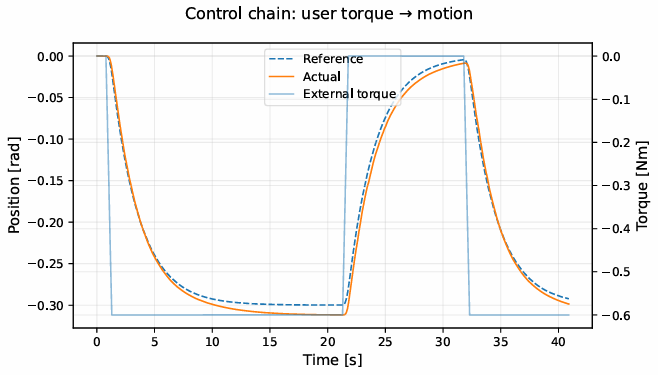
\includegraphics[scale=0.4]{images/chapter4/step_long_combined.png}
    \caption{Step Response}
    \label{fig:step_long_combined}
\end{figure}
\FloatBarrier

\paragraph{Admittance Controller}
Figure~\ref{fig:step_admittance} presents the detailed response of the outer loop. Panel (a) confirms that the input torque is a clean step with a $0.5\;\mathrm{s}$ ramp, free from the configuration-dependent distortion that was observed in preliminary experiments using the Cartesian wrench projection. Panel (b) shows $\theta_v$ reaching the predicted steady state with a rise time (10\%--90\%) of $5.3\;\mathrm{s}$ and a settling time (2\% band) of $9.5\;\mathrm{s}$, both consistent with the dominant pole at $\tau_1 = 2.4\;\mathrm{s}$.

\begin{figure}[ht]
    \centering
    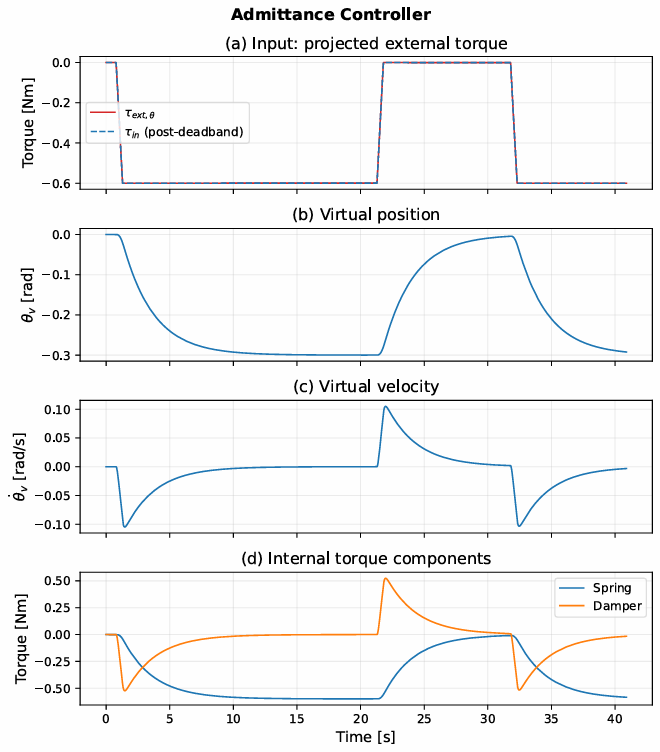
\includegraphics[scale=0.4]{images/chapter4/step_admittance.png}
    \caption{Step Response, admittance control loop}
    \label{fig:step_admittance}
\end{figure}
\FloatBarrier


 
Panel (c) shows the virtual velocity, which peaks at approximately $\pm 0.10\;\mathrm{rad/s}$ during the step edges and decays exponentially to zero during the hold phase. The symmetry between the positive and negative peaks confirms the linearity of the virtual dynamics. Panel (d) shows the internal torque decomposition: the damper component $D_v\dot\theta_v$ dominates during the transient, dissipating the kinetic energy of the virtual system, while the spring component $K_v(\theta_v - \theta_{\mathrm{eq}})$ builds up proportionally to the displacement and alone balances the external input at steady state.

\paragraph{Trajectory Controller}
Figure~\ref{fig:step_trajectory} reports the inner-loop performance. The position tracking error peaks at $0.021\;\mathrm{rad}$ ($\approx 1.2deg$) during the phases of maximum reference velocity and exhibits a root-mean-square value of $0.009\;\mathrm{rad}$ ($\approx 0.5deg$) over the entire experiment. During the hold phase, where the reference is approximately constant, a residual DC error of approximately $0.011\;\mathrm{rad}$ persists. This offset is attributable to the uncompensated Coulomb friction, which acts as an approximately constant disturbance when the velocity is near zero and must be absorbed by the proportional gain, yielding a finite steady-state error $e_\infty \approx f_c / K_p$.

The motor torque remains well within the actuator capacity throughout the experiment. The feed-forward component provides a baseline compensation of the gravitational and passive torques, while the PD component handles the transient tracking effort and the residual disturbances.

\begin{figure}[ht]
    \centering
    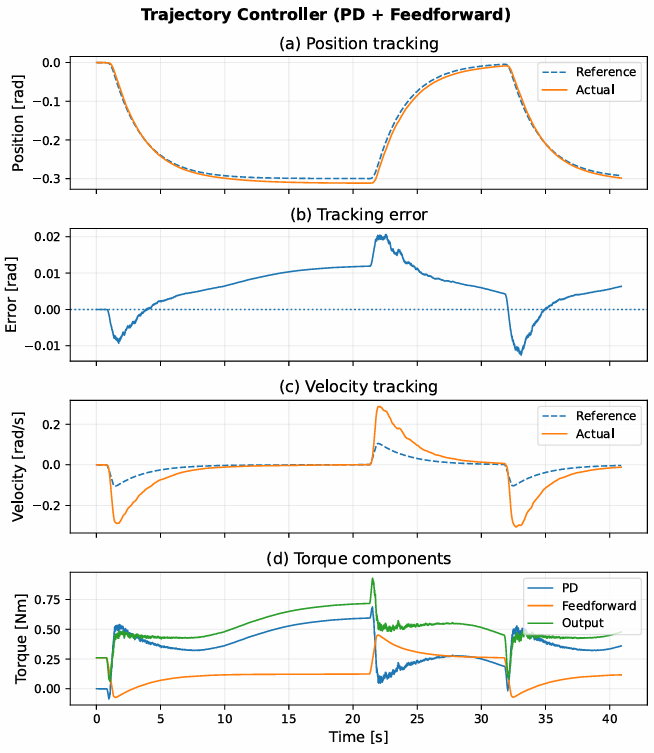
\includegraphics[scale=0.4]{images/chapter4/step_trajectory.png}
    \caption{Step Response, trajectory control loop}
    \label{fig:step_trajectory}
\end{figure}
\FloatBarrier

\subsection{Sinusoidal Response}
The second experiment applies a sinusoidal torque oscillating between $-0.8\;\mathrm{N\,m}$ and $0\;\mathrm{N\,m}$ at a frequency of $f = 0.05\;\mathrm{Hz}$ (period $T = 20\;\mathrm{s}$). This profile approximates the slow, cyclic force pattern that a patient would produce during a flexion--extension rehabilitation exercise, and provides a frequency-domain validation of the cascade architecture complementary to the time-domain step characterisation.

\paragraph{Overall Cascade Response}
Figure~\ref{fig:sine_combined} shows the cascade response after the initial transient. The system reaches a periodic steady state in which both $\theta_{\mathrm{ref}}$ and $\theta$ oscillate smoothly. The measured gain of the cascade - defined as the ratio of the position amplitude to the torque amplitude - is $|\theta/\tau| = 0.40\;\mathrm{rad/Nm}$, which matches the analytical prediction of the virtual admittance transfer function at the excitation frequency within $1\%$:

\begin{equation}
    |G(j\omega)| = \frac{1}{\sqrt{(K_v - M_v\omega^2)^2 + (D_v\omega)^2}} = 0.40\;\mathrm{rad/Nm}
\end{equation}

This close agreement confirms that the inner loop is sufficiently fast to be transparent from the perspective of the outer admittance dynamics: the physical plant behaves as an ideal trajectory follower, and the user perceives the virtual impedance rather than the actual mechanism dynamics.

\begin{figure}[ht]
    \centering
    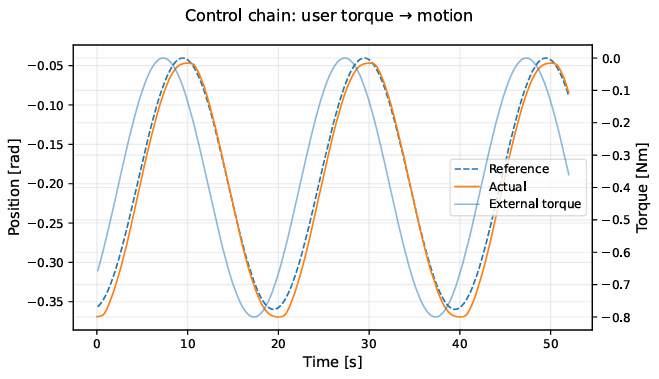
\includegraphics[scale=0.6]{images/chapter4/sine_combined.png}
    \caption{Sine Response}
    \label{fig:sine_combined}
\end{figure}
\FloatBarrier
 
The phase lag between the torque input and the position response is $2.7\;\mathrm{s}$, compared to the analytical prediction of $2.2\;\mathrm{s}$ for the virtual admittance alone. The additional delay of approximately $0.5\;\mathrm{s}$ is attributable to the finite tracking bandwidth of the inner loop, which introduces a phase contribution not captured by the virtual dynamics model.

\subsection{Summary}
The two experiments provide complementary evidence that the cascade control architecture operates as designed. The step response confirms that the admittance controller produces a monotonic, overshoot-free transient with rise and settling times consistent with the overdamped virtual dynamics ($\zeta = 2.5$). The sinusoidal response demonstrates that the cascade gain and phase match the analytical frequency response of the virtual admittance model, with the inner loop introducing a small but measurable additional phase lag. In both cases, the trajectory controller maintains sub-degree position tracking accuracy, and the motor torque remains within the actuator limits.
 
These results validate the proposed Digital Twin (integrating the constrained multibody dynamics, the kinematic closure solver, and the cascade admittance-trajectory control architecture) as a coherent and numerically stable simulation platform for the design and pre-validation of control strategies for the hand exoskeleton.